\documentclass[11pt]{article}
\usepackage[a2paper,margin=1cm]{geometry}
\pagestyle{empty}
\usepackage[T1]{fontenc}
\usepackage{lmodern}
\usepackage{amsmath}
\usepackage{tikz}
\usetikzlibrary{positioning,arrows.meta,fit,backgrounds,calc}

\definecolor{cData} {HTML}{2A78D6}
\definecolor{cFeat} {HTML}{1BAF7A}
\definecolor{cModel}{HTML}{EB6834}
\definecolor{cEval} {HTML}{4A3AA7}
\definecolor{cInk}  {HTML}{0B0B0B}
\definecolor{cMute} {HTML}{52514E}

\begin{document}
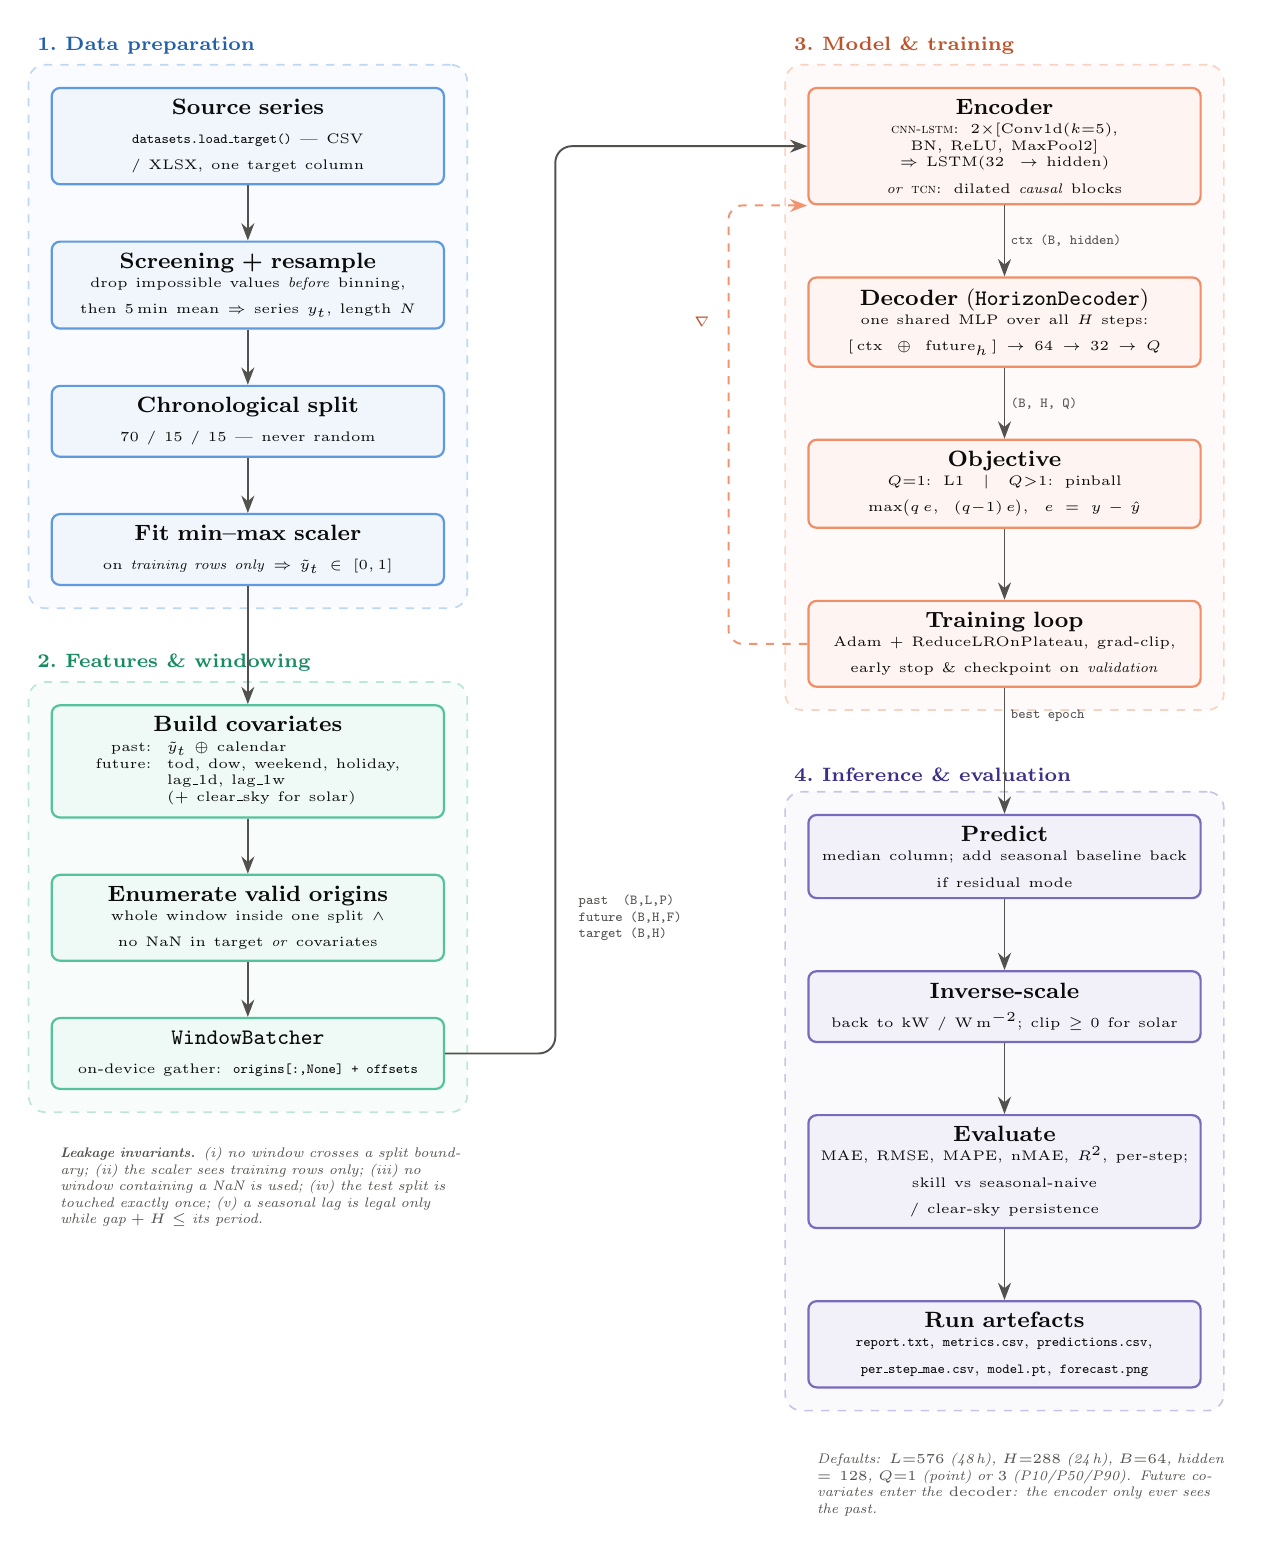
\begin{tikzpicture}[
  >={Stealth[length=2.2mm]},
  node distance=7mm,
  stage/.style={rounded corners=3pt, draw=#1!75, fill=#1!7, line width=0.8pt,
                inner sep=4pt, align=center, text=cInk, font=\footnotesize,
                text width=47mm, minimum height=9mm},
  flow/.style ={->, line width=0.7pt, draw=cMute},
  lbl/.style  ={font=\tiny\ttfamily, text=cMute, inner sep=2pt},
  note/.style ={font=\tiny\itshape, text=cMute, align=left, text width=40mm},
  band/.style ={rounded corners=6pt, draw=#1!30, fill=#1!3, dashed,
                line width=0.6pt, inner sep=8pt},
  bandlbl/.style={font=\scriptsize\bfseries, text=#1!80!black},
]

\node[stage=cData] (src)
  {\textbf{Source series}\\[1pt]
   \tiny\texttt{datasets.load\_target()} --- CSV / XLSX, one target column};

\node[stage=cData, below=of src] (screen)
  {\textbf{Screening + resample}\\[1pt]
   \tiny drop impossible values \emph{before} binning,\\
   then 5\,min mean $\Rightarrow$ series $y_t$, length $N$};

\node[stage=cData, below=of screen] (split)
  {\textbf{Chronological split}\\[1pt]
   \tiny 70 / 15 / 15 --- never random};

\node[stage=cData, below=of split] (scaler)
  {\textbf{Fit min--max scaler}\\[1pt]
   \tiny on \emph{training rows only} $\Rightarrow$ $\tilde y_t\in[0,1]$};

\node[stage=cFeat, below=15mm of scaler] (feat)
  {\textbf{Build covariates}\\[2pt]
   \tiny
   \begin{tabular}{@{}r@{\ \ }l@{}}
     past: & $\tilde y_t\ \oplus$ calendar\\
     future: & tod, dow, weekend, holiday,\\
             & lag\_1d, lag\_1w\\
             & ($+$ clear\_sky for solar)
   \end{tabular}};

\node[stage=cFeat, below=of feat] (orig)
  {\textbf{Enumerate valid origins}\\[1pt]
   \tiny whole window inside one split $\wedge$\\
   no NaN in target \emph{or} covariates};

\node[stage=cFeat, below=of orig] (batch)
  {\textbf{\texttt{WindowBatcher}}\\[1pt]
   \tiny on-device gather: \texttt{origins[:,None] + offsets}};

\node[stage=cModel, right=46mm of src.north east, anchor=north west] (enc)
  {\textbf{Encoder}\\[1pt]
   \tiny \textsc{cnn-lstm}: $2\times$[Conv1d($k{=}5$), BN, ReLU, MaxPool2]\\
   $\Rightarrow$ LSTM($32\to$ hidden)\\
   \emph{or} \textsc{tcn}: dilated \emph{causal} blocks};

\node[stage=cModel, below=9mm of enc] (dec)
  {\textbf{Decoder} (\texttt{HorizonDecoder})\\[1pt]
   \tiny one shared MLP over all $H$ steps:\\
   $[\,\text{ctx}\ \oplus\ \text{future}_h\,]\to 64\to 32\to Q$};

\node[stage=cModel, below=9mm of dec] (loss)
  {\textbf{Objective}\\[1pt]
   \tiny $Q{=}1$: L1\quad$|$\quad$Q{>}1$: pinball\\
   $\max\!\big(q\,e,\;(q{-}1)\,e\big)$, \ $e=y-\hat y$};

\node[stage=cModel, below=9mm of loss] (opt)
  {\textbf{Training loop}\\[1pt]
   \tiny Adam $+$ ReduceLROnPlateau, grad-clip,\\
   early stop \& checkpoint on \emph{validation}};

\node[stage=cEval, below=16mm of opt] (pred)
  {\textbf{Predict}\\[1pt]
   \tiny median column; add seasonal baseline back\\ if residual mode};

\node[stage=cEval, below=9mm of pred] (inv)
  {\textbf{Inverse-scale}\\[1pt]
   \tiny back to kW / W\,m$^{-2}$; clip $\geq 0$ for solar};

\node[stage=cEval, below=9mm of inv] (eval)
  {\textbf{Evaluate}\\[1pt]
   \tiny MAE, RMSE, MAPE, nMAE, $R^2$, per-step;\\
   skill vs seasonal-naive / clear-sky persistence};

\node[stage=cEval, below=9mm of eval] (out)
  {\textbf{Run artefacts}\\[1pt]
   \tiny \texttt{report.txt}, \texttt{metrics.csv}, \texttt{predictions.csv},\\
   \texttt{per\_step\_mae.csv}, \texttt{model.pt}, \texttt{forecast.png}};

\draw[flow] (src)    -- (screen);
\draw[flow] (screen) -- (split);
\draw[flow] (split)  -- (scaler);
\draw[flow] (scaler) -- (feat);
\draw[flow] (feat)   -- (orig);
\draw[flow] (orig)   -- (batch);

\coordinate (gut) at ($(batch.east)+(14mm,0)$);
\draw[flow, rounded corners=6pt]
  (batch.east) -- (gut) -- (gut|-enc.west) -- (enc.west);
\node[lbl, align=left, anchor=west, xshift=2.2mm] at (gut|-orig)
  {past\ \ (B,L,P)\\future\ (B,H,F)\\target\ (B,H)};

\draw[flow] (enc)  -- node[lbl, right] {ctx (B, hidden)} (dec);
\draw[flow] (dec)  -- node[lbl, right] {(B, H, Q)}        (loss);
\draw[flow] (loss) -- (opt);
\draw[flow] (opt)  -- node[lbl, right, pos=0.22] {best epoch} (pred);
\draw[flow] (pred) -- (inv);
\draw[flow] (inv)  -- (eval);
\draw[flow] (eval) -- (out);

\coordinate (bp) at ($(opt.west)+(-10mm,0)$);
\draw[flow, dashed, draw=cModel!70, rounded corners=5pt]
  (opt.west) -- (bp) -- (bp|-enc.south west) -- (enc.south west);
\node[lbl, anchor=east, xshift=-1.6mm, text=cModel!80!black]
  at (bp|-dec) {$\nabla$};

\begin{scope}[on background layer]
  \node[band=cData,  fit=(src)(scaler),   label={[bandlbl=cData ,anchor=south west]north west:1.\ Data preparation}] {};
  \node[band=cFeat,  fit=(feat)(batch),   label={[bandlbl=cFeat ,anchor=south west]north west:2.\ Features \& windowing}] {};
  \node[band=cModel, fit=(enc)(opt),      label={[bandlbl=cModel,anchor=south west]north west:3.\ Model \& training}] {};
  \node[band=cEval,  fit=(pred)(out),     label={[bandlbl=cEval ,anchor=south west]north west:4.\ Inference \& evaluation}] {};
\end{scope}

\node[note, below=6mm of batch.south west, anchor=north west, text width=52mm]
  {\textbf{Leakage invariants.}
   (i) no window crosses a split boundary;
   (ii) the scaler sees training rows only;
   (iii) no window containing a NaN is used;
   (iv) the test split is touched exactly once;
   (v) a seasonal lag is legal only while
   $\text{gap}+H\leq$ its period.};

\node[note, below=7mm of out.south west, anchor=north west, text width=52mm]
  {Defaults: $L{=}576$ (48\,h), $H{=}288$ (24\,h), $B{=}64$,
   hidden $=128$, $Q{=}1$ (point) or $3$ (P10/P50/P90).
   Future covariates enter the \emph{decoder}: the encoder
   only ever sees the past.};

\end{tikzpicture}
\end{document}